\documentclass[../main.tex]{subfiles}
\begin{document}
\section{The Reinforcement Learning Problem}\label{sec:RL}
The following section aims at giving an overview to the standard reinforcement learning problem and methods and is entirely based on the introduction provided in \cite{sutton1998reinforcement}.
Reinforcement learning is a field of machine learning that tackles the problem of how a learning agent should choose actions in order to maximise some notion of cumulative reward. To learn an optimal policy the agent needs to interact with its environment by taking actions and collecting the reward following from these actions. Given a certain state $s_t$, the agent selects an action $a_t$ according to some policy $\pi_t$ and finds itself subsequently in a new state $s_{t+1}$ while receiving some immediate reward $r_{t+1}$. Reinforcement learning algorithms provide different ways of how the agent should modify $\pi$ to maximise its expected return, where the return at time step $t$ is typically defined as
\begin{equation}
R_t = \sum_{k=0}^T \gamma^kr_{t+k+1}.
\end{equation}
In this equation, $T$ describes the horizon of the problem (which could also be $\infty$) and $\gamma \in [0,1]$ denotes the discount factor that can be used to weigh sooner rewards more than later rewards.\par
An important framework to model reinforcement learning problems are Markov Decision Processes (MDP). To model a problem as an MDP, it is necessary that the system fulfills the Markov property. That means that the system response at time $t+1$ only depends on the state and action at time $t$. An MDP is then defined by a quintuple $(S,A,T,r,\gamma$), where $S$ is the state space and $A$ is the action space. $T$ describes the transition probabilities of arriving at a state $s'$ given a state $s$ and an action $a$ i.e. $T(s,a,s') = p(s'|s,a)$. $r(s,a)$ is the reward function that assigns rewards to state $s$ and action $a$ and $\gamma$ is the discount factor that will be further explained below. \par
Given a certain MDP, reinforcement learning algorithms typically try to estimate value functions that describe ``how favourable" a state is, given that starting from that state $s$ a policy $\pi$ is applied. The state-value function under policy $\pi$ (or value function for short) $V^\pi$ is defined in terms of expected return i.e.
\begin{equation}
V^\pi(s) = E_\pi\{R_t|s_t = s\}.
\end{equation}
The value of a state $s$ indicates how favourable that state is. Thus, a higher expected reward implies that a state is more favourable. Alternatively, the value of being in a state $s$, taking an action $a$ and then following a policy $\pi$ is defined by the action-value function
\begin{equation}
Q^\pi(s,a) = E_\pi\{R_t|s_t = s, a_t = a\}.
\end{equation}
This action-value function describes how favourable an state-action pair is. Value functions are used to determine how good a policy is. A policy is better than another, if it achieves a higher expected return for all states and thus has a higher value $V^\pi(s)$ for all $s$. An optimal policy $\pi^*$ is an optimizer to the function
\begin{equation}
V^*(s) = \max_\pi V^\pi(s),
\end{equation}
where $V^*$ is called the optimal state-value function. More formally, $\pi^*$ can be written as:
\begin{equation}
\pi(s)^* \in \text{arg}\max_\pi V^\pi(s).
\end{equation}
The relation between $V^*$ and the action-value function $Q$ can then be expressed as 
\begin{equation}
    V^*(s) = \max_a Q(s,a).
\end{equation}
Given a MDP as defined above, there are algorithms to compute the optimal policy explicitly. The algorithm depends on the formulation of the return $R$. If the horizon over which the return is calculated is finite, the MDP is called a Finite-Horizon MDP and the optimal policy along with its average reward can be computed using Dynamic Programming. If the horizon is infinite and the reward is discounted, i.e. $\gamma<1$, the MDP is called Infinite-Horizon MDP with Discounted Reward. If the reward is undiscounted, the MDP is a Infinite-Horizon MDP with Average Reward and the objective is instead to maximise the average reward. Both classes can be solved with two algorithms, Value Iteration and Policy Iteration. As the MDPs in this thesis are Infinite-Horizon MDPs with Discounted Reward, the solution methods for this class will be explained below.
The first algorithm, Value Iteration, initializes the values of the states randomly and then updates the values each iteration according to the following expression:
\begin{equation}
    V_{k+1}(s) = \max_a \left[ r(s,a) + \gamma  \sum_{s'} T(s,a,s')V_k(s') \right].
\end{equation}
This algorithm is based on the Bellman optimality equations that state
\begin{align}
	V^*(s) &= \max_a E\left\{r_{t+1}+\gamma V^*(s_{t+1}) | s_t = s, a_t = a\right\}\\
	&= \max_a \left[ r(s,a) + \gamma  \sum_{s'} T(s,a,s')V^*(s') \right].
\end{align}
For more details the reader is referred to \cite{sutton1998reinforcement}. Value Iteration can be shown to converge to the optimal policy in polynomial time. As Value Iteration requires an infinite number of steps to converge exactly, the execution of the algorithm is usually stopped when the changes in the values become smaller than some value $\epsilon$.
Policy Iteration works in a similar way but evaluates and improves a policy $\pi$ directly. As the policy usually converges much faster than the values, Policy Iteration gives good results when the actual underlying policy is more important than accurate values.
\subsection{Reinforcement learning algorithms}
Reinforcement algorithms in general try to estimate the value function when the MDP is not entirely known, i.e. transition probabilities and reward function are unknown. There are model-based and model-free algorithms. The former ones try to estimate the underlying model to make it more accrately match the real environment. The latter ones try to obtain the optimal policy directly without approximating the underlying dynamics. All algorithms explained below are model-free. Another important distinction is the one between off-policy and on-policy algorithms. On-policy algorithms update the Q-values according to the policy followed while off-policy learns the optimal Q-values independent of the policy followed. All algorithms explained below except for Delayed Q-Learning are off-policy algorithms.\par
In the following section, some reinforcement learning algorithms are introduced. A classic algorithm in the field of reinforcement learning, known as Q-learning, was presented by Watkins in 1989 \cite{watkins1992q}. In its simplest form the learning update of this algorithm is formulated as
\begin{equation}
Q_{t+1}(s_t,a_t) = Q_{t}(s_t,a_t) + \alpha_t \left[ r_{t+1}+\gamma \max_a Q_{t}(s_{t+1},a) - Q_{t}(s_t,a_t)\right].
\end{equation}
In this expression, $Q_{t+1}$ is the learned action-value function, $\alpha$ is the step size or learning rate, and $r_{t+1}$ is the reward obtained by taking action $a_t$ from state $s_t$ and arriving in the succeeding state $s_{t+1}$.
Per iteration only one state-value pair is updated such that
\begin{equation}
    Q_{t+1}(s,a) = Q_{t}(s,a) \qquad \forall (s,a) \neq (s_t,a_t).
\end{equation}
$Q$ approximates the optimal action-value function $Q^*$. Convergence is ensured as long as the following two conditions on the sequence of step sizes $\alpha$ are fulfilled \cite{jaakkola1994convergence}
\begin{align}\label{eq:stepsize}
    \sum_{t=1}^\infty \alpha_t &= \infty\\
    \sum_{t=1}^\infty \alpha_t^2 &< \infty ,
\end{align}
and all state-action pairs are visited infinitely often as the number of transitions approaches infinity. The former condition is for instance fulfilled with a step size of $\alpha = \frac{1}{n+1}$ where $n$ is the iteration count. The latter condition deals with the trade-off between exploration and exploitation. This describes the need to find a balance between applying the policy that is currently estimated to be best and exploring unknown regions of the state space. One way to ensure this balance is to employ an $\epsilon$-greedy policy that makes the agent choose a random action with probability $\epsilon$ and the action maximising $Q(s,a)$ elsewise. Alternatively, the Q-values could be optimistically initialized to the maximum possible value $V_{\max}$ (for an infinite horizon) that is achieved when the agent would always receive the maximum possible reward. 
\begin{equation}\label{eq:optimistic_init}
    Q_0 = V_{\max} = \sum_{k=0}^\infty \gamma^k\max_{s,a}r(s,a) = \dfrac{\max_{s,a}{r(s,a)}}{1-\gamma}.
\end{equation}
In this case exploration is encouraged because the algorithm will in the beginning of the learning process lower the values from all experienced states and therefore the choice probability of unexplored states increases. \par
Classical Q-learning converges under the above described conditions, but it does so slowly. Therefore, several improvements to the original algorithm have been proposed. Speedy Q-learning is a variant of traditional Q-learning that was introduced in 2011 aimed at increasing the convergence speed \cite{azar2011speedy}. To achieve faster convergence, there are slight changes in the update of the Q-values. Instead of only taking the Q-function of the current iteration into account, the update incorporates also the previous Q-function. The learning update becomes
\begin{multline}
Q_{t+1}(s_t,a_t) = Q_{t}(s_t,a_t) + \alpha_k \left[ r_{t+1}+\gamma \max_a Q_{t-1}(s_{t+1},a) - Q_{t}(s_t,a_t)\right] \\+ (1-\alpha_k) \left[ r_{t+1}+\gamma \max_a Q_{t}(s_{t+1},a) -  r_{t+1}+\gamma \max_a Q_{t-1}(s_{t+1},a)\right].
\end{multline}
The second term goes to zero as the Q-values converge to the optimal values. Therefore, the usual step size conditions do not need to be fulfilled for this term and the algorithm achieves a larger step size while still ensuring convergence. More detailed convergence results can be found in \cite{azar2011speedy}.\par
Another variation of Q-learning is the Delayed Q-learning algorithm for the online problem. The most major change compared to traditional Q-learning is that the Q-values are only updated after $m$ samples are collected so that the update rule becomes
\begin{equation}\label{DelayedQ}
Q_{t+1}(s_t,a_t) = \dfrac{1}{m} \sum_{i=1}^m \left( r_{k_i} + \gamma \max_{a} Q_{k_i}(s_{k_i},a) \right) + \varepsilon
\end{equation}
where $m$ and $\varepsilon$ are inputs to the algorithm. The algorithm is designed such that for an update to be performed, the change in the Q-value has to be larger than $2\varepsilon$, where $\varepsilon \in (0,1)$. Furthermore, the number of attempted updates is limited such that after the update of a state-action pair's Q-value has been attempted $m$ times a successful update of any Q-value has to occur until the update is attempted again. It is then possible to obtain PAC-MDP guarantee \cite{strehl2006pac}, where PAC stands for Probably Approximately Correct. This guarantee implies that with high probability an upper bound holds on the sample complexity, i.e. the number of time steps that the agent executes a policy whose value at the current state is not $\epsilon$-close to that of the optimal policy. The details of the convergence proof can be found in \cite{strehl2006pac}.\par
A different approach to Q-learning for large state and action spaces is Q-learning with function approximation. In this method, information from a limited subset of the state space is generalised to cover the whole state space.  In case of linear function approximation the Q-function becomes
\begin{equation}
Q_\theta(s,a) = \sum_{i=1}^n \theta_{i,a}\varphi_i(s) = {\theta}^{\,T} \varphi
\end{equation}
where $\theta$ is the parameter matrix and $\varphi$ is the vector of basis functions. $\varphi_i$ can for instance be chosen to be a Gaussian radial basis function
\begin{equation}
\varphi_i(s) = \text{exp}\left(\dfrac{-||s-m_i||^2}{2\sigma_i^2}\right)
\end{equation}
where $m_i$ is the center and $\sigma_i$ is the standard deviation of the resulting Gaussian function. These parameters need to be tuned in order for the function approximation to accurately approximates the true function. For instance, the standard deviation of the basis functions determines which distance generalization takes place over. In the $t$-th iteration of the learning process, a gradient-descent update of one column of the parameter matrix can then be performed in each iteration:
\begin{align}
\delta_t &= r_{t+1} + \gamma \max_a Q_\theta(s_{t+1},a) - Q_\theta(s_{t},a_t)\\
\theta_{\bullet,a_{t+1}} &= \theta_{\bullet,a_{t}} + \alpha \cdot \delta_t  \cdot \varphi_t(s_t).
\end{align}
A detailed convergence analysis of this method can be found in \cite{tsitsiklis1997analysis}.


\section{Gaussian Processes for Regression}
The following introduction to Gaussian processes (GP) is based on \cite{murphy2012machine} and \cite{rasmussen2006gaussian}. Generally, GPs are powerful non-parametric methods that can be applied for regression and classification. Our specific interest lies in applying GPs to a number of collected data points and obtain an upper and lower bound for a disturbance. Model fitting is a typical application of GP regression. The striking advantage of GP regression in our application is that we not only obtain an estimate for the disturbance, but also a measure for the certainty of this estimate. This enables us to choose upper and lower disturbance bounds that hold with a very high probability. A more formal introduction to GP regression is given in the following. In \cite{rasmussen2006gaussian}, GPs are defined to be a ``collection of random variables, any finite number of which have (consistent) joint Gaussian distributions". GP can be understood as the generalization of Gaussian distributions to a continuous input space and thus an infinite number of random variables. While Gaussian distributions are over finite-dimensional vectors and defined by a covariance matrix and a mean vector, GPs are over functions and defined by a mean function and a covariance function.\par
GPs can be applied for regression in the following manner. A GP 
\begin{equation}
    f(x) \sim GP(m(x),\kappa(x,x'))
\end{equation}
with mean function $m(x)$ and positive definite covariance function $\kappa(x)$ can be used as a prior for Bayesian inference. Then, a set of known function values $\mathbf{f}$ associated with training inputs $\mathbf{X}$, and a set of unknown function values $\mathbf{f^*}$, associated with test inputs $\mathbf{X^*}$, are according to the definition above jointly Gaussian distributed. Formally, this can be written as
\begin{equation}
    \left(
    \begin{array}{c}
      \mathbf{f(\mathbf{X})} \\\mathbf{f(\mathbf{X^*})}
    \end{array}
 \right) \sim \mathcal{N}
 \left(\left( 
  \begin{array}{c}
  \boldsymbol{\mu} \\ \boldsymbol{\mu}_* 
  \end{array}
  \right),
  \left(\!
  \begin{array}{c}
  \mathbf{K} \hspace{0.5cm} \mathbf{K}_* \\
  \mathbf{K}^T_* \hspace{0.5cm} \mathbf{K}_{**}  
  \end{array}
  \right)
  \right)
\end{equation}
with $\mathbf{K} = \kappa(X,X)$, $\mathbf{K_*} = \kappa(X,X_*)$ and $\mathbf{K_{**}} = \kappa(X_*,X_*)$. For predicting values for the test inputs $\mathbf{f}_*$, the conditional distribution of $\mathbf{f}_*$ given $\mathbf{f}$ can be calculated to be
\begin{align}
    p(\mathbf{f}_*|\mathbf{X}_*,\mathbf{X},\mathbf{f}) &= \mathcal{N}(\mathbf{f}_*|\boldsymbol{\mu}_*,\boldsymbol{\Sigma}_*)\\
    \boldsymbol{\mu}_* &= \boldsymbol{\mu}(\mathbf{X}_*)+\mathbf{K}^T_*\mathbf{K}^{-1}(\mathbf{f}-\boldsymbol{\mu}(\mathbf{X}))\\
    \boldsymbol{\Sigma}_* &= \mathbf{K}_{**} - \mathbf{K}^T_*\mathbf{K}^{-1}\mathbf{K}_*.
\end{align}
The result does not only give a prediction of the unknown function values (the test means) but also a measure of how reliable this prediction is (the test variance). An important result is that the function interpolates the data points exactly in case of noiseless function outputs. An example for a Gaussian prior and a Gaussian posterior conditioned on noisefree data can be seen in figure $\ref{fig:GP_example}$. In the lower figure it is evident that the confidence in the prediction decreases with increasing distance to a datapoint.\par

\begin{figure}
    \centering
    \begin{subfigure}[b]{\textwidth}
    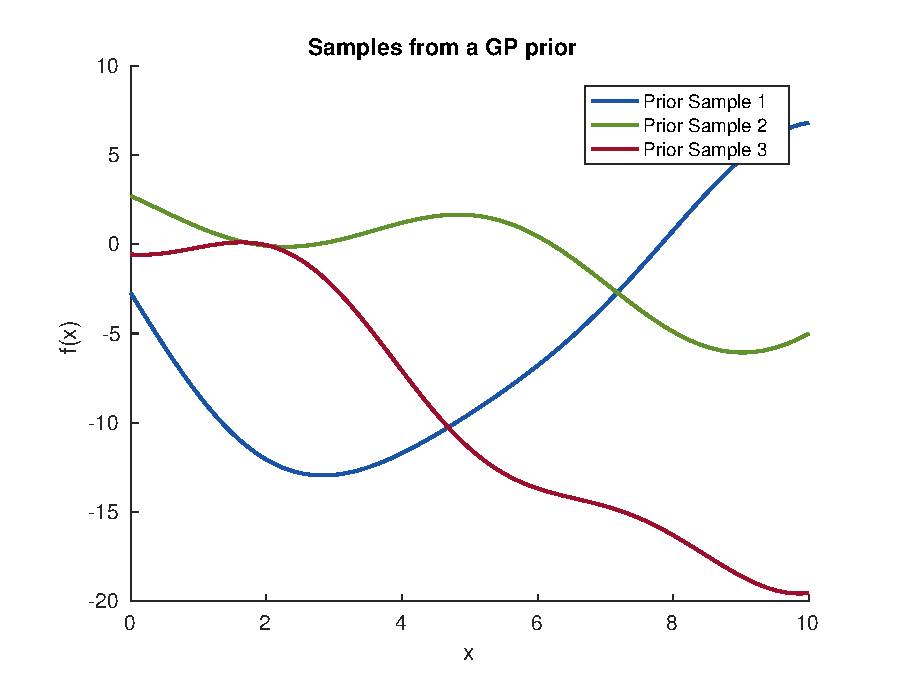
\includegraphics[width=\textwidth]{GaussianProcess_example_prior}
    \end{subfigure}
    
    \begin{subfigure}[b]{\textwidth}
    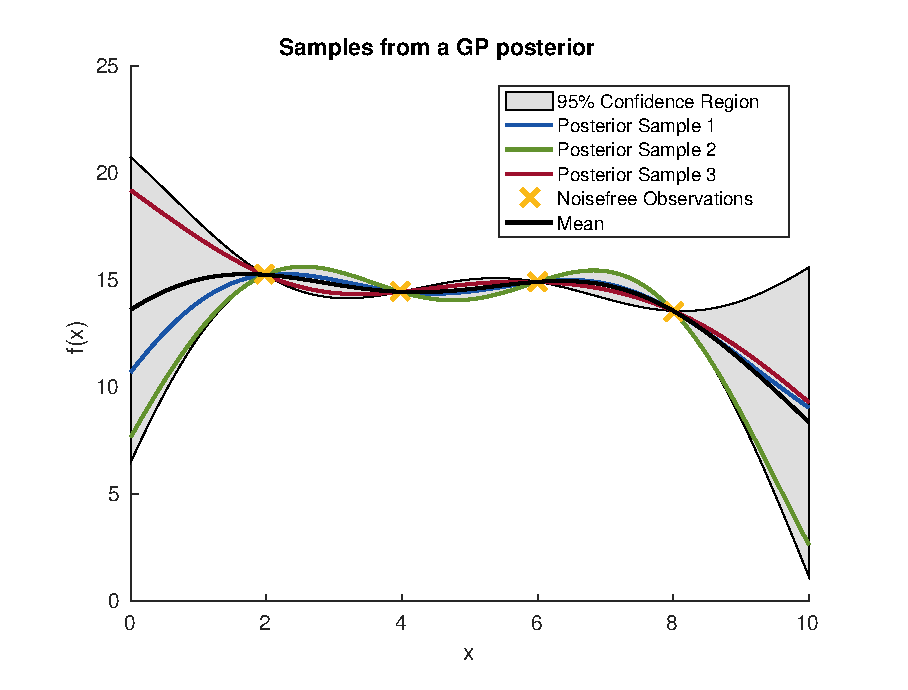
\includegraphics[width=\textwidth]{GaussianProcess_example}
    \end{subfigure}
    \caption{The upper figure shows samples from a Gaussian prior with a squared exponential kernel. The lower figure shows samples from the Gaussian posterior conditioned on four noisefree observations (yellow). Additionally, the mean function (black) and the $\pm 2 \sigma$-confidence region (grey) is shown.}    
    \label{fig:GP_example}
\end{figure}

If the function outputs are corrupted with Gaussian noise, the covariance function of the training inputs is no longer $\mathbf{K}$ but
\begin{equation}
    \mathbf{K}_y = \mathbf{K} + \sigma_y^2\mathbf{I}_N
\end{equation}
where $\sigma_y^2$ is the covariance function of the independently added noise. In this case the model does not exactly interpolate the observed data points.\par
Covariance and mean functions determine some function properties such as smoothness. The mean function is often chosen to be zero as the GP model is flexible enough to still model the function arbitrarily well. A widely employed covariance function that results in a smooth function is the squared exponential kernel:
\begin{equation}\label{eq:sqexp}
    \kappa(x,x') = \sigma^2_f \text{ exp}(-\dfrac{1}{2l^2}(x-x')^2).
\end{equation}
This kernel reflects the intuition that ``nearby inputs" should map to ``nearby outputs". \par 
An important question is how the kernel parameters $l$,$\sigma_f$ and $\sigma_n$ should be chosen. The horizontal length scale $l$ determines the horizontal scale of the function, i.e. how ``wiggly" the signal looks. The signal standard deviation $\sigma_f$ is a vertical length scale and defines how much the signal deviates from the mean. The noise standard deviation $\sigma_n$ describes how much noise is expected to be present in the data. If $\sigma_n = 0$ the data points are noiseless and will be fitted exactly. \par
In this section the estimation of the hyperparameters $\theta = \{l,\sigma_f, \sigma_n\}$ by maximizing the marginal likelihood will be explained. Generally, the goal is to find the set of hyperparameters that explains the obtained data points in the best possible way or more formally, maximises the probability $p(y|x,\theta)$. The corresponding log-likelihood function is given by
\begin{align}
    L(y|X, \theta) &= \log p(y|x,\theta) = \log \mathcal{N}(0,\mathbf{K}_y)\\
    &= -\dfrac{1}{2} \log|\mathbf{K}_y|-\dfrac{1}{2}y^T\mathbf{K}_y^{-1}y-\dfrac{n}{2}\log(2\pi),
\end{align}
where $N$ is the dimension of the data set. The first part of the formula corresponds to a complexity penalty term, whereas the second term is a data-fit measure. This property is of great importance as it implies that a trade-off between complexity and data-fit is automatically introduced and does not need to be tuned manually \cite{rasmussen2006gaussian}. 
Maximising the likelihood function can be done based on the derivative
\begin{equation}
    \frac{\partial L}{\partial \theta_i} = \dfrac{1}{2} \text{ trace} \left( \mathbf{K}_y^{-1} \frac{\partial \mathbf{K}_y}{\partial \theta_i} \right) + \frac{1}{2}y^T\mathbf{K}_y^{-1} \frac{\partial \mathbf{K}_y}{\partial \theta_i} \mathbf{K}_y^{-1} y.
\end{equation}
Given this expression, the kernel parameters can be estimated with standard gradient-based optimizers. Since the objective is however not guaranteed to be convex, local minima can pose problems.


\section{Safe Set Computations based on Reachability Analysis}\label{sec:SafeSets}
This section aims at giving a brief explanation of a method known as Hamilton-Jacobi-Isaacs (HJI) reachability analysis that is employed in this thesis to guarantee safety within the learning framework. Both explanation and implementation are based on Ian M. Mitchell's Level Set Toolbox \cite{mitchell2004toolbox} and doctoral thesis \cite{mitchell2003application}.

Guaranteeing safety in our context means to ensure that a disturbed system will never leave a safe region $\mathcal{S}_0$. To this end, we assume that the disturbance $d$ lies within a set $\mathcal{D}$ and a set $\mathcal{U}$ is given in which one can choose a control $u$. The question is now in which set $\mathcal{S}_\tau$ the initial conditions must lie such that there is a control strategy that makes the system stay in $\mathcal{S}_0$ within the time horizon $t \in [-\tau,0]$. 

As we require safety for all possible trajectories, it is not sufficient to simulate a few thousands or even millions trajectories, because there still is a risk to miss an unsafe trajectory. Instead, one can compute the backwards reachable set of the unsafe set $\mathcal{T}_0 = \mathbb{R}^n\backslash \mathcal{S}_0$ to capture all possible trajectories at once. To this end, we assume a control that tries to steer the system away from the unsafe set and an adversarial disturbance that tries to steer the system into the unsafe set. The backwards reachable set $\mathcal{T}_\tau$ is the set from which trajectories start that can reach the unsafe set within the time horizon $\tau$ and should therefore be avoided for all $t \in [-\tau,0]$. Figure \ref{fig:reachable} illustrates this concept. Safety could therefore be guaranteed for time horizon $\tau$, if we had a way to calculate the set $\mathcal{T}_\tau$ and a control strategy to stay outside that set. 

\begin{figure}
    \centering
    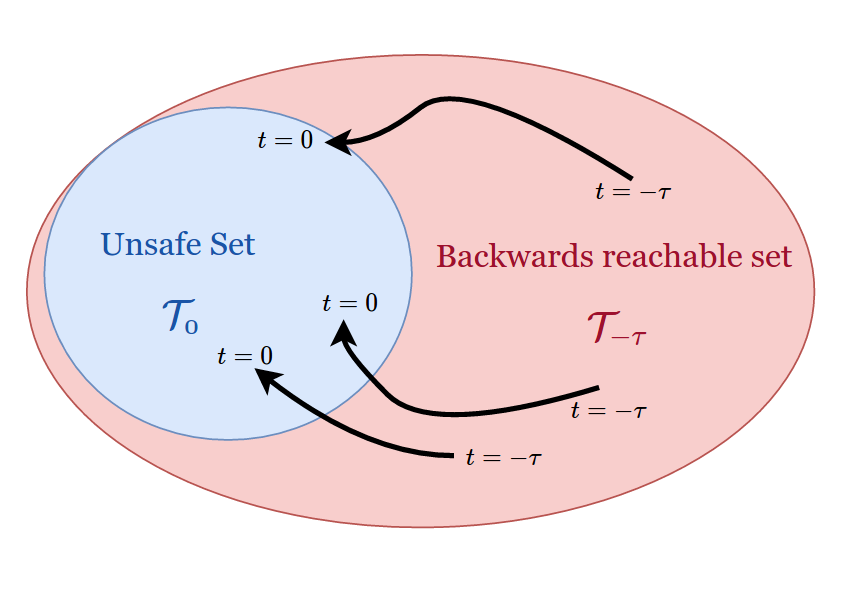
\includegraphics[width=\textwidth]{ReachableSet.png}
        \caption{The backwards reachable set $\mathcal{T}_\tau$ is the set from which trajectories can reach the unsafe set within time $\tau$.}    
    \label{fig:reachable}
\end{figure}
The present section aims at showing a way as to how one can obtain both, the backwards reachable set and the safety-preserving control strategy, by solving the time-dependent HJI partial differential equation (PDE). The unsafe set $\mathcal{T}_0$ can be represented as the zero sublevel set of a bounded and Lipschitz continuous function $g: \mathbb{R}^n \rightarrow \mathbb{R}$, namely
\begin{equation}
    \mathcal{T}_0 = \left\{ x \in \mathbb{R}^n | g(x) \leq 0 \right \}. 
\end{equation}
We can then calculate the backwards reachable set as the viscosity solution \linebreak \mbox{$\phi: \mathbb{R}^n \times [-T, 0] \rightarrow \mathbb{R}$} of the time dependent HJI PDE
\begin{align}
    \frac{\partial}{\partial t} \phi(x,t) + \min\left[0, H\left(x,\frac{\partial}{\partial x} \phi(x,t)\right)\right] = 0, \qquad &\forall t \in [-T, 0], \forall x \in \mathbb{R}^n\\
    \phi(x,0) = g(x), \qquad &\forall x \in \mathbb{R}^n
\end{align}
where $H(x,p)$ is the Hamiltonian: 
\begin{equation}\label{eq:hamil}
    H(x,p) = \max_{u \in \mathcal{U}} \min_{d \in \mathcal{D}} p^T f(x,u,d).
\end{equation}
The function $f(x,u,d)$ in this expression describes the system dynamics.

While the sublevel set of $\phi(x,0)$ corresponds to the unsafe set $\mathcal{T}_0$ as stated above, the sublevel set of $\phi(x,t)$ describes the backwards reachable set $\mathcal{T}_\tau$:
\begin{equation}
    \mathcal{T}_\tau = \left\{ x \in \mathbb{R}^n | \phi(x,t) \leq 0 \right \}, \qquad \forall \tau \in [0,T].
\end{equation}
There are well-established numerical methods to accurately approximate $\phi(x,t)$ and thereby $\mathcal{T}_\tau$ even for non-linear dynamics. It can then be guaranteed that for states outside the backwards reachable set, there exists a control $u \in \mathcal{U}$ for all $d \in \mathcal{D}$ to keep the system outside the unsafe set for a time horizon $\tau$. More specifically, it is sufficient to apply the optimizer $u_{\text{safe}}$ of $\eqref{eq:hamil}$ given by
\begin{equation}
    u_{\text{safe}} = \arg \max_{u \in \mathcal{U}} \min_{d \in \mathcal{D}} p^T f(x,u,d)
\end{equation}
whenever the system hits the boundary of the safe set. Within the safe set $\mathcal{S}_\tau$, the control can be freely chosen e.g. by a learning controller. 
Furthermore, the backwards reachable set typically converges for a sufficiently large $\tau$ so that safety can then be guaranteed by staying within the control-invariant set $\mathcal{S}_\tau$ for all time. 

\end{document}
